\documentclass{../slides}

\title{3827 OH}
\author{Eumin Hong (eh2890)}
\institute{Columbia University}
\date{February 22, 2022}

\begin{document}

\begin{frame}
    \titlepage
\end{frame}

\begin{frame}{Overview}
\begin{multicols}{2}
\tableofcontents
\end{multicols}
\end{frame}

\section{Announcements}
\subsection{Upcoming Assessments}
\begin{frame}{\secname: \subsecname}
    \begin{itemize}
        \item For HW4, do not hand in \enquote{Warmup Problems}
        \item HW4 is due on Friday 2/25
        \item HW2 is graded
    \end{itemize}
\end{frame}

\subsection{Homework 2 Feedback}
\begin{frame}{\secname: \subsecname}
    \begin{itemize}
        \item Common errors from Homework 2:
        \begin{itemize}
            \item Neither $AB + \overbar{A}\overbar{B}$ nor $A\overbar{B} + \overbar{A}B$ are equal to a constant $0$ or $1$ (XNOR and XOR respectively)
            \item SoP and PoS forms must be logically equivalent -- PoS is not the negation of SoP form, but can be found by negating twice
            \item Don't cares do not have to be included when choosing prime implicants (hence their name)
        \end{itemize}
    \end{itemize}
\end{frame}

\begin{frame}{\secname: \subsecname\ (cont.)}
    \begin{multicols}{2}
    \begin{itemize}
        \item Common errors from Homework 2 (cont.):
        \begin{itemize}
            \item Filling in K-maps:
            \begin{karnaugh-map}[4][4][1][$CD$][$AB$]
                \manualterms{0,1,2,3,4,5,6,7,8,9,10,11,12,13,14,15}
            \end{karnaugh-map}
        \end{itemize}
        \item I did not comment much on the PIs/EPIs part of problem 7 -- please look at the solutions for this
    \end{itemize}
    \end{multicols}
\end{frame}

\subsection{Feedback}
\begin{frame}{\secname: \subsecname}
    \begin{itemize}
        \item Form: \url{https://forms.gle/cnUmKVNYN7WvRbHA6}
    \end{itemize}
\end{frame}

\section{Homework 4 Warmup}
\subsection{Problem 1}
\begin{frame}{\secname: \subsecname}
    Build
    \begin{enumerate}[(a)]
        \item a $T$ flip-flop out of a $D$ flip-flop and combinational circuitry.
        \item a $D$ flip-flop out of a $T$ flip-flop and combinational circuitry.
    \end{enumerate}
\end{frame}

\subsection{Problem 2}
\begin{frame}{\secname: \subsecname}
    Build a sequential circuit that returns $1$ whenever the last $3$ inputs (INCLUDING the current input) were identical.
\end{frame}

\subsection{Problem 3}
\begin{frame}{\secname: \subsecname}
    Build a sequential circuit that returns $1$ whenever the last $3$ inputs (PRIOR to the current input) were identical.
\end{frame}

\section{Homework 4 Harder Problems}
\subsection{Problem 1}
\begin{frame}{\secname: \subsecname}
    A special flip-flop is formed from three latches, arranged in sequence. The first two latches behave as in a normal flip-flop: the leader latch’s enable is attached to the clock, and the followers enable is attached to the complement of the clock. The third latch, which follows the follower, is also attached to the clock. What's different about the outputs of this flip-flop?
\end{frame}

\subsection{Problem 2}
\begin{frame}{\secname: \subsecname}
    Design a circuit using $JK$ flip-flops that takes in a binary stream $B_0B_1B_2B_3\cdots$ and outputs a $1$ at time $t$ if the streams received thus far (i.e., $B_0B_1\cdots B_{t-1}B_t$), when read as an unsigned binary number from low bit to high, is divisible by $3$.

    The following table depicts a sample input stream and what should be output.
    \begin{figure}[H]
        \centering
        \begin{tabular}{|c||c|c|c|c|c|c|c|c|c|}\hline 
            $t$ & $0$ & $1$ & $2$ & $3$ & $4$ & $5$ & $6$ & $7$ & $8$ \\\hline
            $In(t)$ & $0$ & $0$ & $1$ & $1$ & $0$ & $0$ & $1$ & $0$ & $0$ \\\hline
            Val of input & $0$ & $0$ & $4$ & $12$ & $12$ & $12$ & $76$ & $76$ & $76$ \\\hline
            Val mod $3$ & $0$ & $0$ & $1$ & $0$ & $0$ & $0$ & $1$ & $1$ & $1$ \\\hline
            Output & $1$ & $1$ & $0$ & $1$ & $1$ & $1$ & $0$ & $0$ & $0$ \\\hline
        \end{tabular}
    \end{figure}
\end{frame}

\begin{frame}{\secname: \subsecname\ (cont.)}
    Hint: The value of the new bit starts as equal to $1$ which is $1\mod 3$, then is $2$ which is $2\mod 3$, then is $4$ which is back to $1\mod 3$, etc.
    \begin{enumerate}[(a)]
        \item Draw the state machine, numbering your states in an \enquote{obvious} manner. You may assume that the machine starts in the right state at time $t=0$.
        \item Give the algebraic formula (simplified as much as possible) for the $J$ and $K$ inputs of your flip-flops, and also for the output.
    \end{enumerate}
\end{frame}

\subsection{Problem 3}
\begin{frame}{\secname: \subsecname}
    Consider a sequential circuit that reads in an input $X(t)$ during clock cycle $t$. The circuit should look for the sequence $011$. Design the sequential circuit (i.e., give simplified algebraic expressions) using $D$ flip-flops for each of the following versions:
    \begin{enumerate}[(a)]
        \item If the second $1$ arrives during clock cycle $t$, then the circuit should output a $1$ during clock cycle $t$, and otherwise outputs a $0$.
        \item If the second $1$ arrives during clock cycle $t$, then the circuit should output a $1$ during clock cycle $t+1$, and otherwise outputs a $0$.
        \item Suppose the sequence is $111$ instead of $011$. If at time $t$, the current and two previous inputs were all $1$, then a $1$ should be output during clock cycle $t$, and otherwise a $0$ should be output. Note that multiple consecutive outputs of $1$ are possible.
    \end{enumerate}
\end{frame}

\section{Homework 4 Topics}
\subsection{SR Latch}
\begin{frame}{\secname: \subsecname}
    \begin{itemize}
        \item Latches just hold state -- can be changed by changing the values of the inputs
        \item SR latch has inputs of \enquote{Set} ($S$) and \enquote{Reset} ($R$)
        \item SR latch has outputs of $Q$ and $\overbar{Q}$
    \end{itemize}
    \begin{figure}[H]
        \centering
        \begin{tikzpicture}[circuit logic US, label distance=2mm]
            \node (r) at (0, 3) {$R$};
            \node (s) at (0, 0) {$S$};
            \node[nor gate, draw] (n1) at (2, 2.5) {};
            \node[nor gate, draw] (n2) at (2, 0.5) {};
            \node (q) at (4.5, 2.5) {$Q$};
            \node (q') at (4.5, 0.5) {$\overbar{Q}$};
            \draw (n1.output) -- (q) ;
            \draw (n2.output) -- (q') ;
            \draw (r) --(1, 3) |- (n1.input 1);
            \draw (s) --(1, 0) |- (n2.input 2);
            \draw (3.5, 2.5) -- (3.5, 2.25) -- (1, 1) |- (n2.input 1);
            \draw (3.5, 0.5) -- (3.5, 0.75) -- (1, 2) |- (n1.input 2);
            \draw[black,fill=black] (3.5, 2.5) circle (0.05) node[anchor=south east] {};
            \draw[black,fill=black] (3.5, 0.5) circle (0.05) node[anchor=south east] {};
        \end{tikzpicture}
    \end{figure}
    \begin{itemize}
        \item For understanding behavior of circuit for given $(R, S)$, think about when NOR operation gives $0$
        \begin{itemize}
            \item Or more generally, passing a constant to a gate can make its output constant as well
        \end{itemize}
    \end{itemize}
\end{frame}

\subsection{D Latch}
\begin{frame}{\secname: \subsecname}
    \begin{itemize}
        \item Basically SR latch with some more circuitry to avoid \enquote{illegal} combinations of inputs (e.g. when $R = 1, S = 1$ what does the SR latch do? How can it \enquote{set} $Q = 1$ and \enquote{reset} $Q = 0$ at the same time?)
        \item D latch has inputs $D$ and $C$ (control, which ensures $S\neq R$ in the underlying SR latch)
        \begin{itemize}
            \item $D$ is the value to store/write if $C = 1$
            \item $C$ can also be $E$ for enable
        \end{itemize}
    \end{itemize}
\end{frame}

\subsection{Clocking}
\begin{frame}{\secname: \subsecname}
    \begin{multicols}{2}
        \begin{itemize}
            \item Clock signal oscillates between $0$ and $1$ with a fixed period
            \begin{itemize}
                \item \enquote{Rising edge} of clock signal is the transition from \enquote{low} to \enquote{high} (i.e. $0\to 1$)
            \end{itemize}
            \begin{figure}[H]
                \centering
                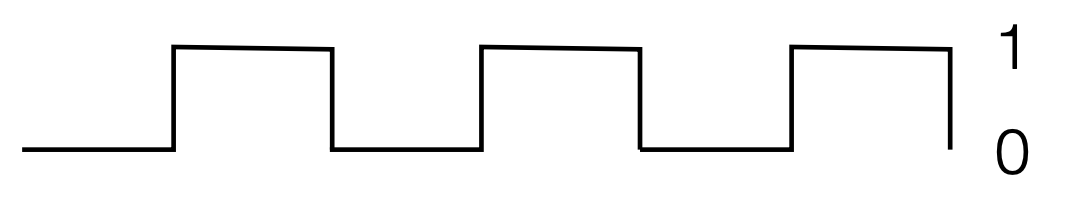
\includegraphics[width = 4cm]{img/clock.png}
            \end{figure}
            \begin{itemize}
                \item Kind of like a metronome, gives the circuit a sense of time on which it can operate
            \end{itemize}
            \begin{itemize}
                \item Why should I care about clock? It determines the rate at which instructions are executed
            \end{itemize}
            \begin{figure}[H]
                \centering
                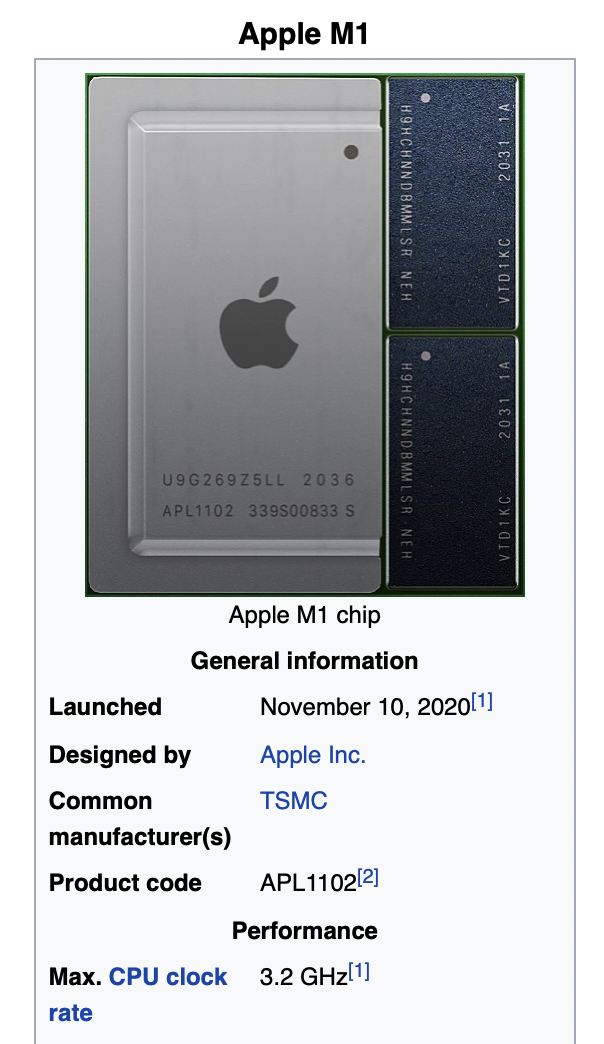
\includegraphics[width = 4cm]{img/m1.png}
            \end{figure}
        \end{itemize}
    \end{multicols}
\end{frame}


\subsection{Flip-Flops}
\begin{frame}{\secname: \subsecname}
    \begin{itemize}
        \item Latches do not support clocking individually
        \item Connecting latches in series (and ensuring that the clock inputs are complemented or staggered) acts as a flip-flop
        \item Example of D Flip-Flop:
        \begin{figure}[H]
            \centering
            \tikzset{flipflop DC/.style={flipflop, flipflop def={t1=D, t2=C, t6=Q, t4={\ctikztextnot{Q}}}}}
            \begin{tikzpicture}[circuit logic US, label distance=2mm]
                \node[flipflop DC] (D1) at (0, 0) {};
                \node[flipflop DC] (D2) at (4, 0) {};
                \node (s) at (-3, 0.84) {$S$};
                \node (c) at (-3, 0) {$CLK$};
                \node (q) at (6, 0.84) {$Q$};
                \node (q') at (6, -0.84) {$\overbar{Q}$};
                \node[not gate, draw] (not) at (0, -2) {};
                \draw (s) -- (D1.pin 1);
                \draw (c) -- (D1.pin 2);
                \draw (D1.pin 6) -- (D2.pin 1);
                \draw (D2.pin 6) -- (q);
                \draw (D2.pin 4) -- (q');
                \draw (-2, 0) |- (not.input);
                \draw (not.output) -| (2, 0) -- (D2.pin 2);
                \draw[black,fill=black] (-2, 0) circle (0.05) node[anchor=south east] {};
            \end{tikzpicture}
        \end{figure}
        \item Left D latch is updated when $CLK = 1$ (new inputs read to left D latch), right D latch is updated when $CLK = 0$ (load new inputs to right D latch)
    \end{itemize}
\end{frame}

\subsection{Flip-Flop Behavior}
\begin{frame}{\secname: \subsecname}
    \begin{itemize}
        \item For the D flip-flop:
        \begin{figure}[H]
            \centering
            \begin{tabular}{c|c}
                $D(t)$ & $Q(t + 1)$\\\hline
                $0$ & $0$ \\
                $1$ & $1$
            \end{tabular}
        \end{figure}
        \item The input $t$ is time, or more specifically, the $t$th clock cycle
        \begin{itemize}
            \item A clock cycle is one period of the clock
        \end{itemize}
        \item In other words, the input $D$ at clock cycle $t$ becomes the output $Q$ at clock cycle $t+1$ (the next clock cycle)
    \end{itemize}
\end{frame}

\subsection{Flip-Flop Abstraction}
\begin{frame}{\secname: \subsecname}
    \begin{itemize}
        \item The two latch circuit from earlier is abstracted and is a D flip-flop (D since it has the same inputs as a D latch) (left circuit)
        \begin{figure}[H]
            \centering
            \begin{tikzpicture}[circuit logic US, label distance=2mm]
                \node[flipflop D] () at (0, 0) {};
                \node[flipflop D, add async SR] () at (4, 0) {};
            \end{tikzpicture}
        \end{figure}
        \item The triangular input (bottom left) is for the clock signal
        \item How do we initialize the values of a flip-flop?
        \begin{itemize}
            \item Use set and reset inputs (right circuit), implementation is not necessary to know (we are not really worried about initialization in this course)
        \end{itemize}
    \end{itemize}
\end{frame}

\subsection{State Machines}
\begin{frame}{\secname: \subsecname}
    \begin{itemize}
        \item We will worry about Mealy form -- output is based on input and state, rather than just state
        \item Let the inputs be $I = I_{n-1}I_{n-2}\cdots I_1I_0$ and the outputs be $O = O_{m-1}O_{m-2}\cdots O_1O_0$
        \item Then, for every state in the FSM, there must be $2^{n}$ transitions accounted for, each corresponding to $I_{n-1}I_{n-2}\cdots I_1I_0 / O_{m-1}O_{m-2}\cdots O_1O_0$ (but replace with $0$s and $1$s, so something like $01\cdots 00 / 11\cdots 10$)
        \begin{itemize}
            \item Why $2^{n}$? Because every combination of inputs must appear exactly once for each state since we will deal with deterministic FSMs
        \end{itemize}
    \end{itemize}
\end{frame}

\begin{frame}{\secname: \subsecname\ (cont.)}
    \begin{itemize}
        \item Example: $I = I_1I_0$, $O = O_0$
        \begin{figure}[H]
            \centering
            \begin{tikzpicture}
                \node[state] (a) at (0, 0) {$A$};
                \node[state] (b) at (4, 4) {$B$};
                \node[state] (c) at (8, 0) {$C$};
                \draw[-{Stealth[scale=1.5]}] (a) edge[bend left = 15] node[in place] {$00/1$} (b);
                \draw[-{Stealth[scale=1.5]}] (a) edge[bend left = 15] node[in place] {$1X/0$} (c);
                \draw[-{Stealth[scale=1.5]}] (a) edge[loop below] node[in place] {$01/0$} (a);
                \draw[-{Stealth[scale=1.5]}] (b) edge[bend left = 15] node[in place] {$X0/0$} (c);
                \draw[-{Stealth[scale=1.5]}] (b) edge[bend left = 15] node[in place] {$X1/0$} (a);
                \draw[-{Stealth[scale=1.5]}] (c) edge[loop below] node[in place] {$1X/1$} (c);
                \draw[-{Stealth[scale=1.5]}] (c) edge[loop right] node[in place] {$00/0$} (c);
                \draw[-{Stealth[scale=1.5]}] (c) edge[bend left = 15] node[in place] {$01/1$} (b);
            \end{tikzpicture}
        \end{figure}
    \end{itemize}
\end{frame}

\subsection{FSM to Circuits}
\begin{frame}{\secname: \subsecname}
    \begin{itemize}
        \item High-level approach to go from problem to circuit
        \begin{enumerate}
            \item FSM
            \item Truth table in terms of just current state bits and next state bits
            \item Add columns for flip-flops to go from state bit $A(t)$ to next state bit $A(t+1)$
            \item Derive K-maps for each output (overall output and flip-flop inputs)
            \item Boolean expression
            \item Circuit
        \end{enumerate}
        \item Choice of flip-flop
        \begin{itemize}
            \item D flip-flops results in fewer outputs/K-maps
            \item JK flip-flops results in simpler expressions
            \item You will be told which flip-flop to use
        \end{itemize}
    \end{itemize}
\end{frame}

\end{document}
